\documentclass[12pt,a4paper,openany]{extarticle}
% подключаем собственный стилевой файл
\usepackage{mystyle}
\selectlanguage{russian}
\graphicspath{{./pictures/}}
\usepackage[pdftex]{lscape}
\usepackage{graphicx}
\usepackage{systeme}

\begin{document}

\section{Теоретические сведения\\}

\paragraph*{Параметры Денавита-Хартенберга\\}

\hspace*{\parindent}Как известно, для определения любого трехмерного тела в пространстве достаточно задать ему 6 координат (3 координаты перемещения и 3 координаты вращения). Для оптимизации задачи описания положения тела, существует метод, позволяющий сократить число необходимых координат до 4 - метод Денавита - Хартенберга.\\

\hspace*{\parindent}Координаты, позволяющие описать положение тела данным методом называются параметрами Денавита-Хартенберга:
\begin{enumerate} 
 \item[1.] Координатами $a_i$ - обозначаются расстояния по осям $x_i$ (текущая ось) от  $z_{i-1}$ до $z_i$;
 \item[2.] Координаты $\alpha_i$ - обозначают угол вращения оси $x_i$ (текущая ось) от  $z_{i-1}$ до $z_i$;
 \item[3.] Координатами $d_i$ - обозначаются расстояния по осям $z_{i-1}$ (предыдущая ось) от  $x_{i-1}$ до $x_i$;
 \item[4.] Координаты $\theta_i$ - обозначают угол вращения оси $z_{i-1}$ (предыдущая ось) от  $x_{i-1}$ до $x_i$.\\
 \end{enumerate}
 
 \paragraph*{Определение систем координат\\}
 
\hspace*{\parindent}Для удобного определения осей в каждом звене есть несколько правил:
\begin{enumerate} 
\item[1.] Ось $z_i$ выбирается как сонаправленная с осью вращения(движения) $i+1$ сочленения. Далее расположение смежных звеньев будет определяться именно положением этой оси.
\item[2.] Для оси $x_i$ существуют два условия: ось $x_i$ перпендикулярна оси $z_{i-1}$ и пересекает её при мысленном продолжении. (Для упрощения задачи желательно, чтобы в начальных(нулевых) конфигурациях оси $x_{i-1}$ и $x_i$ были сонаправлены.)
\item[3.] Ось $y_i$ задается согласно принципу правой тройки векторов, чтобы выполнялось тождество ($y_i = z_i x x_i$).
 \end{enumerate}

(КАРТИНКИ С ОСЯМИ)\\

\begin{center}
    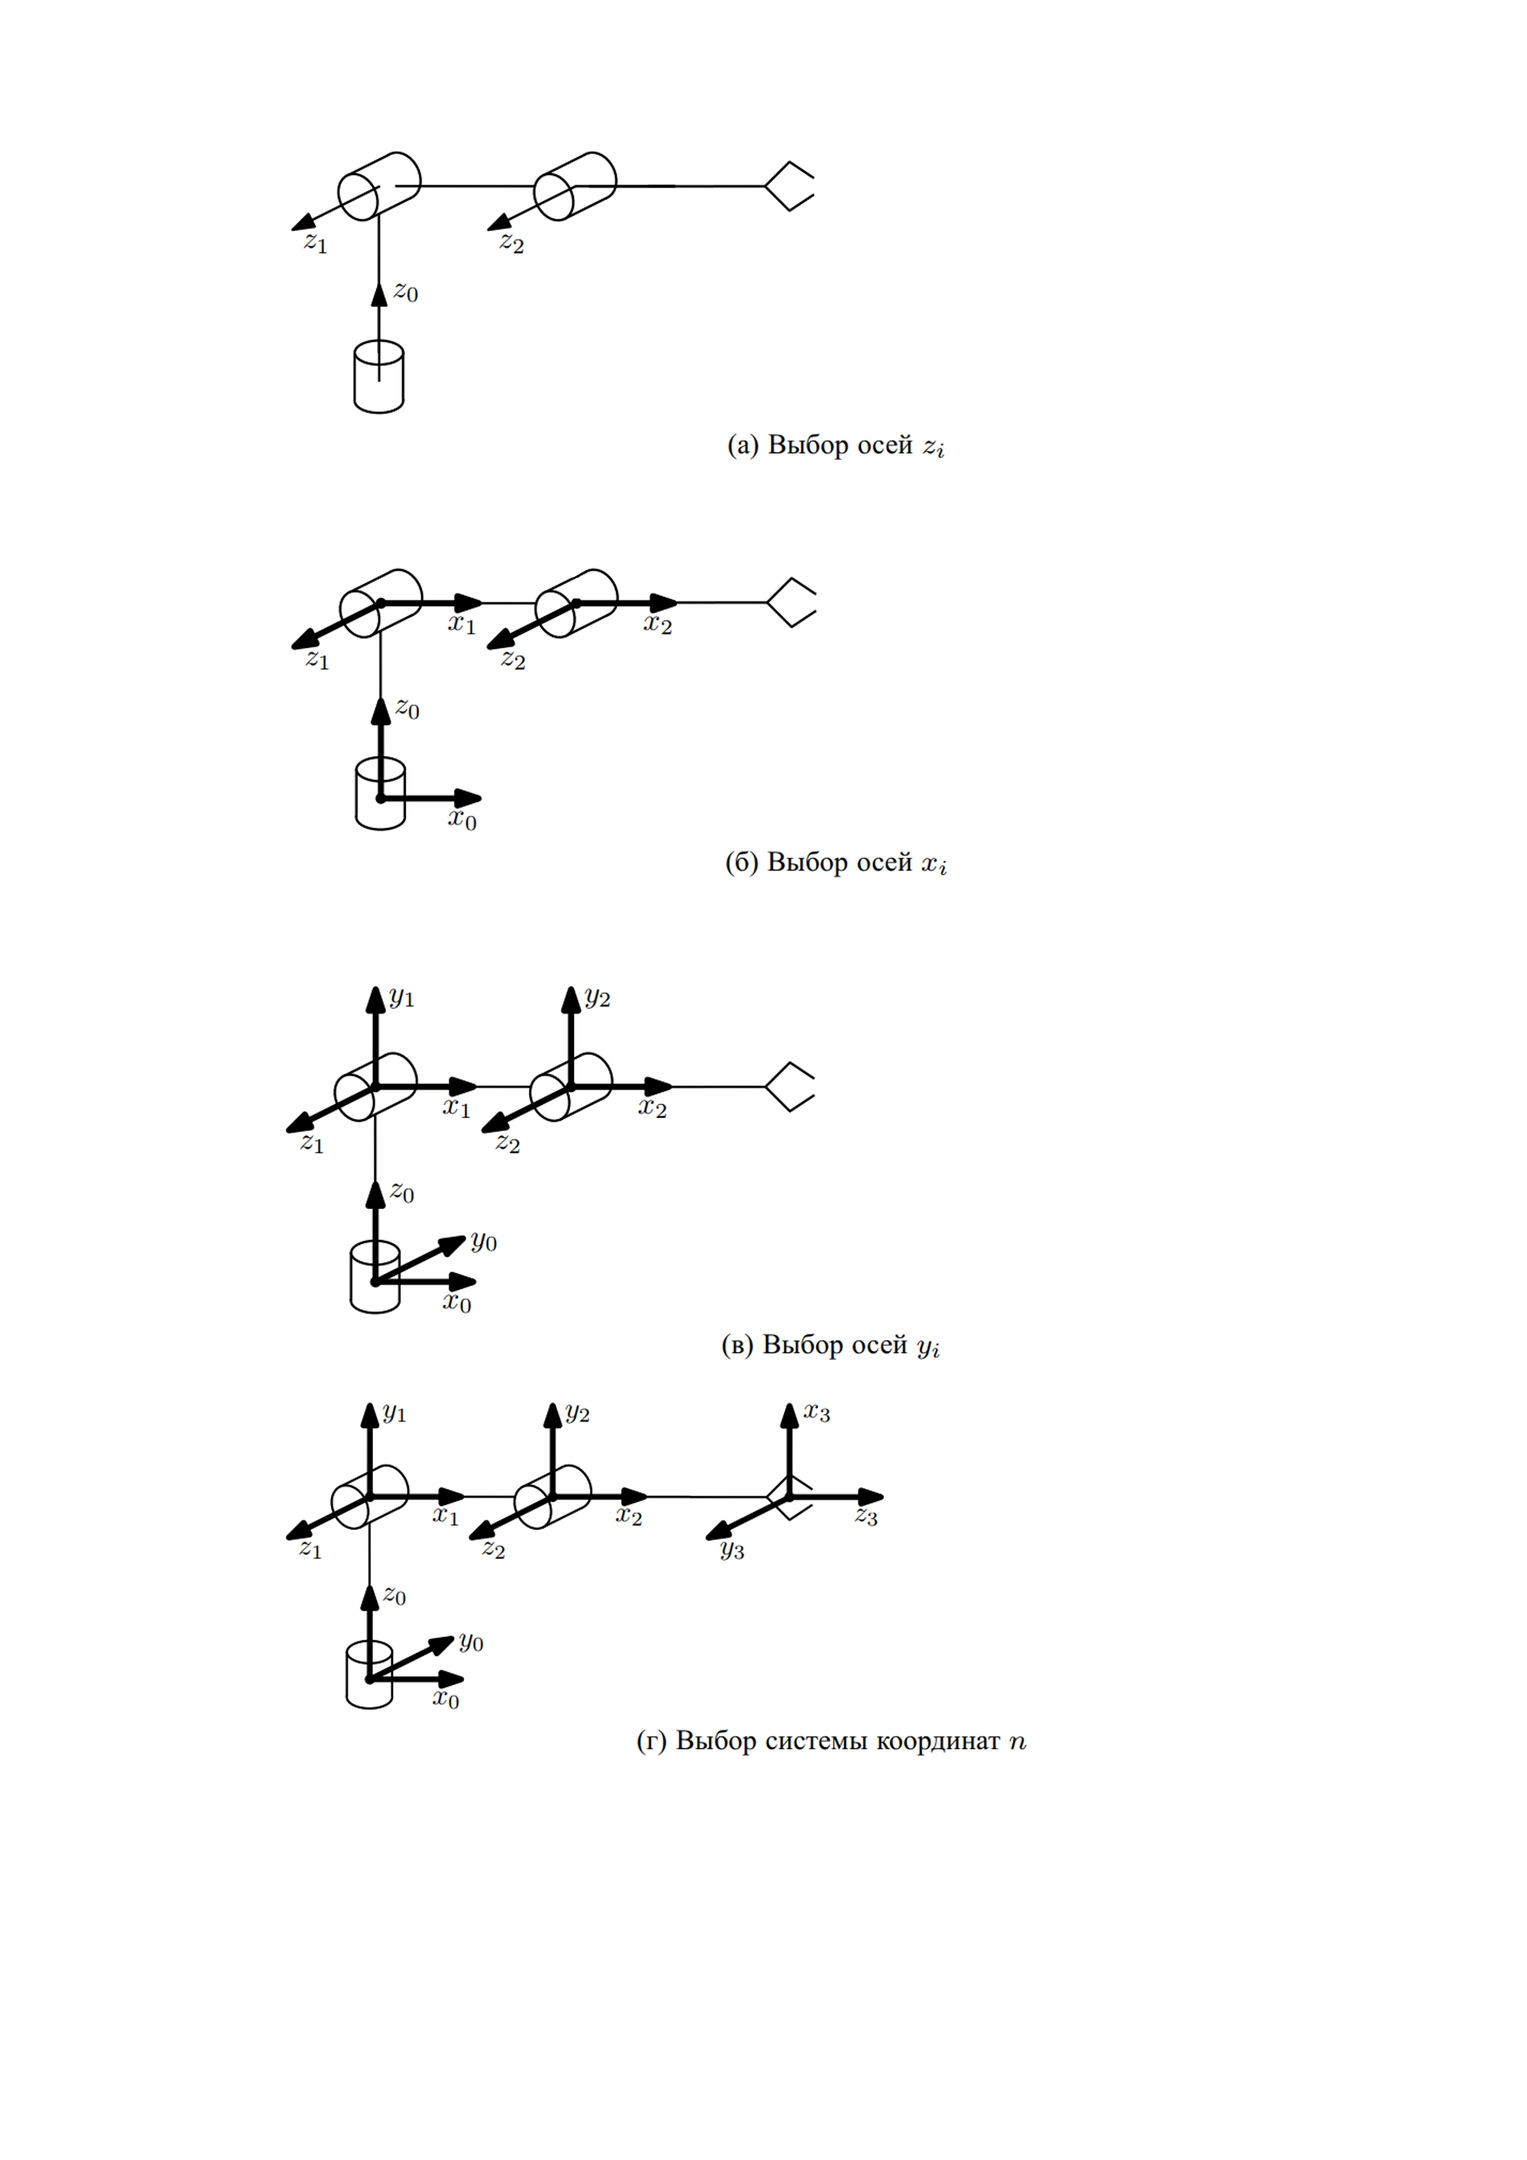
\includegraphics[width=\textwidth]{axes.jpg}\\
\end{center}

\hspace*{\parindent}Как ранее говорилось, вначале выбираются значения осей $z_i$: ось вращения первого звена будет проходить через ось изображаемого цилиндра, т.к. вращение происходит в этой плоскости, аналогично выбираются оси для остальных звеньев вращения, также можно заметить, что можно было выбрать направление осей $z_1$ и $z_2$ "от нас", но это  ухудшает наглядность схемы, поэтому выбирается направление "на нас". Оси $x_i$ выбираются по принципу перпендикулярности к соответствующим осям $z_i$, и направленные на пересечение с последующими из них, так выбрано направление "вправо" в первом звене и сонаправленном с ним втором для нулевого параметра начального угла в параметрах DH. Далее не происходит только смещение по оси перпендикулярной оси вращения, поэтому направление осей $x_i$ остаётся неизменным. Оси $y_i$ достраиваются в соответствии с правилом правой тройки векторов (можно использовать и левую, что приведёт к некотором изменениям знаков в дальнейших преобразованиях, но наиболее используемой является правая). Система последнего звена получается путём смещения на некоторое расстояние, поскольку схват и его сочленения статичны.\\
 
 \paragraph*{Практическая часть\\}
 
\hspace*{\parindent}Рассмотрим нахождение этих параметров на конкретной задаче:\\
(КАРТИНКИ С ПАРАМЕТРАМИ)\\

\hspace*{\parindent}После того, как были получены значения, достаточные для описания положения тела в пространстве, можно приступать к задачам нахождения связи между обобщенной системы координат манипулятора и системы координат, связанной со схватом (рабочим инструментом). Для этого будут использованы матричные преобразования систем координат.\\

\end{document}








 
 
 
